% ****** Start of file apssamp.tex ******
%
%   This file is part of the APS files in the REVTeX 4.1 distribution.
%   Version 4.1r of REVTeX, August 2010
%
%   Copyright (c) 2009, 2010 The American Physical Society.
%
%   See the REVTeX 4 README file for restrictions and more information.
%
% TeX'ing this file requires that you have AMS-LaTeX 2.0 installed
% as well as the rest of the prerequisites for REVTeX 4.1
%
% See the REVTeX 4 README file
% It also requires running BibTeX. The commands are as follows:
%
%  1)  latex apssamp.tex
%  2)  bibtex apssamp
%  3)  latex apssamp.tex
%  4)  latex apssamp.tex
%
\documentclass[%
 reprint,
%superscriptaddress,
%groupedaddress,
%unsortedaddress,
%runinaddress,
%frontmatterverbose, 
%preprint,
%showpacs,preprintnumbers,
%nofootinbib,
%nobibnotes,
%bibnotes,
 amsmath,amssymb,
 aps,
%pra,
%prb,
%rmp,
%prstab,
%prstper,
%floatfix,
]{revtex4-1}

\usepackage[T1]{fontenc}
\usepackage[utf8]{inputenc}
\usepackage{graphicx}% Include figure files
\usepackage{dcolumn}% Align table columns on decimal point
\usepackage{bm}
\usepackage{siunitx}% bold math
%\usepackage{hyperref}% add hypertext capabilities
%\usepackage[mathlines]{lineno}% Enable numbering of text and display math
%\linenumbers\relax % Commence numbering lines

%\usepackage[showframe,%Uncomment any one of the following lines to test 
%%scale=0.7, marginratio={1:1, 2:3}, ignoreall,% default settings
%%text={7in,10in},centering,
%%margin=1.5in,
%%total={6.5in,8.75in}, top=1.2in, left=0.9in, includefoot,
%%height=10in,a5paper,hmargin={3cm,0.8in},
%]{geometry}

\begin{document}

\preprint{APS/123-QED}

\title{Adversarial Examples}% Force line breaks with \\
%\thanks{A footnote to the article title}%

\author{Jan Plank}
\email{janhendrik.plank@stud.uni-goettingen.de}
% \altaffiliation[Also at ]{Physics Department, XYZ University.}%Lines break automatically or can be forced with \\
\author{Philipp Höhne}%
 \email{philipp.hoehne@stud.uni-goettingen.de}
%

%\collaboration{MUSO Collaboration}%\noaffiliation

\author{Jonas Dehning}
\email{j.dehning@stud.uni-goettingen.de}
\affiliation{
Universität Göttingen
}%

\date{\today}% It is always \today, today,
             %  but any date may be explicitly specified

\begin{abstract}
In this work we generated adversarial examples for convolutional networks trained on two different data sets. Two different methods were compared for their generation: the first is to add a small ``noise'' in the direction of the gradient of the loss function, the other is to minimize a custom function which allows to find an example closer to the original image than with the gradient method. Then the robustness of the networks to adversarial examples were compared for the two data sets as function of the depth of networks.


%\begin{description}
%\item[Usage]
%Secondary publications and information retrieval purposes.
%\item[PACS numbers]
%May be entered using the \verb+\pacs{#1}+ command.
%\item[Structure]
%You may use the \texttt{description} environment to structure your abstract;
%use the optional argument of the \verb+\item+ command to give the category of each item. 
%\end{description}
\end{abstract}

%\pacs{Valid PACS appear here}% PACS, the Physics and Astronomy
                             % Classification Scheme.
%\keywords{Suggested keywords}%Use showkeys class option if keyword
                              %display desired
\maketitle

%\tableofcontents

\section{Introduction}

Convolutional neural networks for classifying images are already used by a large number of companies, by Facebook to identify faces or Tesla to recognize people crossing the street in front of the car. 
However these neural networks are vulnerable to adversarial examples, meaning that they misclassify some images which are only slightly different to correctly classified ones. In many cases different machine learning techniques, even if trained on different subsets of the training data, misclassify the same adversarial examples \cite{paperGrad}. Thus adversarial examples seem to reveal a fundamental weakness of those machine learning techniques. Furthermore this suggests that these techniques are unable to learn the true underlying concepts for the correct classification, although they perform extremely well on the training data. They work well for naturally occurring data but fail if they visit points in space that are unlikely to occur in the data. This is problematic for computer vision where it is assumed that the Euclidean distance approximates the perceptual distance.

In course of the increasing use of neural networks the understanding of their weaknesses is of growing interest. To be able to better understand the effects of adversarial examples on neural networks one first has to find ways how to create these. That's why we tested two different methods on two different data sets. Furthermore we analyzed how the robustness of our networks depends on the depth of the network.

\subsection{Convolutional Neural Networks}


In this analysis we only used convolutional neural networks. They are composed of successive convolutional and pooling layers. In the convolutional layer each pixel (neuron) gets the input of the surrounding pixels of the previous layer or the image, and multiply it by a matrix, thus making a convolution. The convolutional matrix is the same for the whole image but typically for each convolutional layer a set of matrices are used, each one applied to the whole image. The results of the different convolutions are set as input for different ``maps'' in a convolutional layer. Between convolutional layers, pooling layers are inserted. They reduce the number of the previous by taking the maximum of a square of 2x2 pixels in our case. To counterbalance the reduced resolution the number of pixels, the number of maps of the following convolutional layers are increased.

At the end some fully connected layers are inserted. There every neuron is connected to every neuron from the previous layer.

This sort of network mimic the visual areas of the brain. There neurons typically respond to a small region of the visual field called receptive field. The size of the receptive fields increase in areas higher in the visual hierarchy, like in a convolutional network with pooling layers.

\subsection{The Data Sets}

We used two different data sets. The first is the MNIST data set downloaded from \emph{kaggle.com}, which contains a little more than 40,000 greyscale images of handwritten digits. Each image has $28\times 28$ pixels, resulting in a 784 dimensional vector representing one image. 

The second data set is a selection from the Asirra data set provided by \emph{kaggle.com} for the ``Dogs vs. Cats'' challenge. It contains 25,000 colored images of dogs and cats of different sizes. That's why we rescaled them to $128\times 128$ pixels each. With 3 color channels this leads to a 49,152 dimensional vector representing each image. 
\section{Methods}

\subsection{The used networks}

We trained for each dataset three different networks, that differed in the number of the convolutional layers. Their exact design is described in the appendix. They are based on networks published on the Kaggle website. The training was done with the Adam optimizer, with a learning rate of \SI{1e-3}{} for the MNIST networks and \SI{1e-4}{} for the Dogs vs Cats networks. The training was interrupted when the loss function of the validation set, consisting of \SI{20}{\percent} of the pictures didn't decrease for 5 respectively 3 epochs. 
We used the Keras library with the Tensorflow backend to generate the networks.

\subsection{Methods for creating adversarial examples}

There are various ideas that have already been used to create adversarial examples. In this project we followed the propositions of \citeauthor{paperGrad} who created a noise in the direction of the gradient of the loss function and \citeauthor{paperMinimize} who proposed to minimize the L2-norm of the noise under misclassification.
\subsubsection*{Gradient method}
In this method a noise is created in the direction of the gradient with the given formula:
\begin{align*}
\vec{\eta} = \epsilon \cdot \operatorname{sign} \left( \nabla_{\vec{x}} J_{loss} \big \vert_{\vec{x}} \right)
\end{align*}
with the noise $\vec{\eta}$, the image $\vec{x}$, the loss function of the neural network $J_{loss}$ for the true category, the gradient regarding the pixel input $\nabla_{\vec{x}}$ and a constant factor $\epsilon$.\\
The label with the smallest value of the loss function $J_{loss}$ will be predicted by the neural network. The idea is to perturb the image in a way to increase this value for the true prediction in order to decrease the possibility, that the true label will be predicted. In order to achieve this one perturbs the image in direction of the gradient of the loss function with respect to the image input as this the direction in with the loss function will most increase. As the size of the gradient can vary strongly one uses just the direction and perturbs with a fixed ratio $\epsilon$. \cite{paperGrad}
\subsubsection*{Minimize method}
This method is based on the one presented on the method by \citeauthor{paperMinimize}, who proposed to minimize the L2-norm of the noise under the constrain, that the network performs a misclassification. As this is computationally very expensive, as this needs to be done individually for each label, in order to find the global minimum, we came up with the idea to minimize the L2-norm while minimizing the prediction of the true label, hence maximizing the loss function. In order to do this at the same time we came up with the following
\begin{align}
\min_{\vec{\eta}} \left( c \cdot \sigma(\vec{\eta}) + \frac{1}{1 + \delta - p(\vec{x}+\vec{\eta})} \right) & \label{eq:minimize}\\
\end{align}
with the noise $\vec{\eta}$, the image $\vec{x}$, the standard deviation of the noise $\sigma (\vec{\eta})$, a scaling factor $c$ and a small factor $\delta$. As the goal is to minimize the L2-norm we chose the standard deviation to keep this formula scalable for different input dimensions (which is the L2-norm divided by square root of N). To minimize the prediction one could just simply add the prediction linearly, however better results were accomplished but adding the nonlinearity of $1/(1-p)$, as predictions close to one (which are unwanted) are stronger panelized. However as $p$ can reach a value of $1$ the function $1/(1 + \delta - p)$ was chosen with $\delta \ll 1$ in order to prevent devision by zero. The scaling constant $c$ is used to keep the two different parts in balanced. Unfortunately those where found to be not completely independent of the input dimensions, however just a factor of 10 apart for the MNIST and the dogs vs cats networks. For the MNIST networks a scaling factor of $c = 100$ and for dogs vs cats networks a scaling factor of $c = 1000$ was used. Those were found by a rough linear minimization.

\subsection{Hypothesis}

How robust a network is to adversarial examples is no easy task to predict, especially since the origin of adversarial examples is still under debate. \citet{paperGrad} argues that adversarial can be explained by linear behavior in high-dimensional spaces and that most neural networks are kept near the linear regime for training purposes. Following this argumentation one has to expect that neural networks with a high-dimensional input will be more vulnerable to adversarial examples.
On the other side it is well known that the spatial gradient is decreasing for an increasing number of layer. This phenomenon is known as the \emph{vanishing gradient problem}. Since the adversarial example is nothing more than a noise added to a training example, the prediction error depends on how much this noise is changing the loss function. This is reflected by the gradient. Thus our assumption is, that a smaller gradient should lead to a more robust network and that a smaller gradient is equivalent to a deeper network.



\section{Results}

\subsection{Comparison of the methods}

\begin{figure}
\centering
\showthe\columnwidth
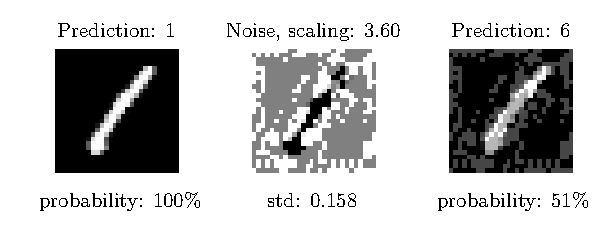
\includegraphics[width = 1\linewidth]{figures/mnist_model2_I0_f0277.pdf}
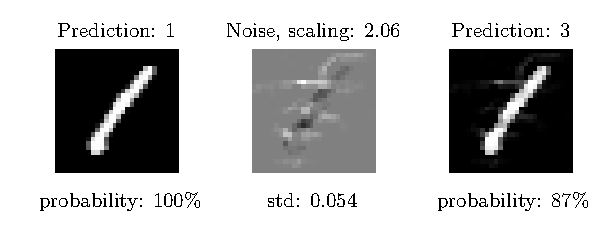
\includegraphics[width = 1\linewidth]{figures/adv_example_minimizer_mnist_0.pdf}
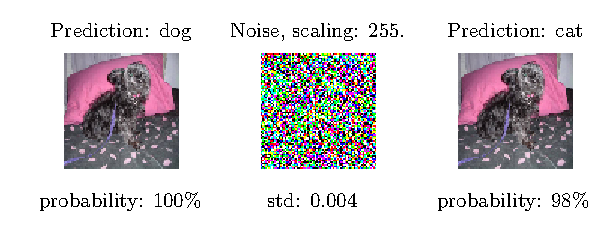
\includegraphics[width = 1\linewidth]{figures/cvd_model9_I0_f0003.pdf}
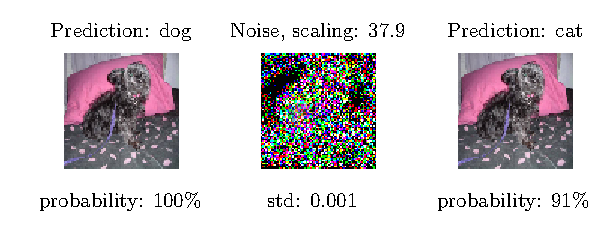
\includegraphics[width = 1\linewidth]{figures/adv_example_minimizer_dogs_vs_cats_0.pdf}
\caption{Adversarial examples created with the two methods using the two different networks. Top two: network trained using the MNIST dataset; bottom two: network trained using the dogs vs cats dataset. For each first: created using the gradient method, second: created using the minimize method. The left and right images range from 0 to 1 for 0 dark to 1 full intensity, while the image of the noise scales from negative to positive values evenly as the noise can also be negative.}
\label{fig:examples}
\end{figure}


In the figure \ref{fig:examples} different examples of adversarial examples, created with the two different methods are shown. We remark that the standard deviation of the examples created with the minimizer method are smaller than the onces created with the gradient method. Both methods can be proven to create adversarial examples.\\

\begin{figure}
\centering
\showthe\columnwidth
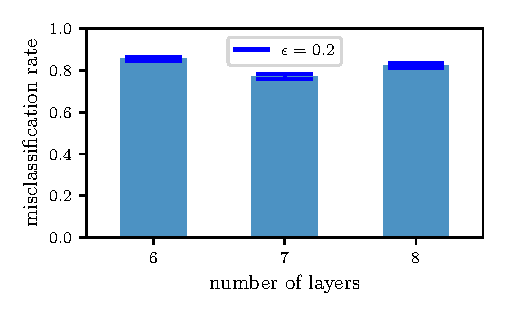
\includegraphics[width = 1\linewidth]{figures/mnist_grad_misclassificationrate.pdf}
\caption{The misclassification rate of different networks for adveraerial examples created with the gradient method with a fixed $\epsilon$ of 0.2 for the MNIST dataset.}
\label{fig:comp_grad_mnist}
\end{figure}

\begin{figure}
\centering
\showthe\columnwidth
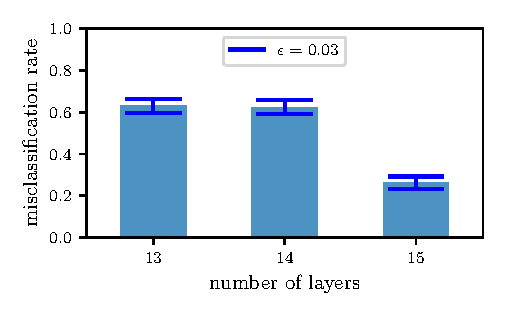
\includegraphics[width = 1\linewidth]{figures/cvd_grad_misclassificationrate.pdf}
\caption{The misclassification rate of different networks for adversarial examples created with the gradient method with a fixed $\epsilon$ of 0.03 for the Cats vs Dogs dataset.}
\label{fig:comp_grad_cats_vs_dogs}
\end{figure}

As described in section \ref{sec:} neural networks are likely to become more robust with higher depth. In order to investigate this neural networks with one convolutional layer more and one convolutional layer less compared to the above used have been created and trained on the same datasets. To compare the robustness for the gradient method, the number of misclassifications (number of successful adversarial examples) for a fixed $\epsilon$ was calculated for a set of images. If the network gets more robust towards adversarial examples with higher depth, the misclassification rate should decrease. In figure \ref{fig:comp_grad_mnist} this was plotted for the MNIST networks. The predicted trend could not be validated in this case. In figure \ref{fig:comp_grad_cats_vs_dogs} this was plotted for the dogs vs cats networks, where this trend is visible. \\

\begin{figure}
\centering
\showthe\columnwidth
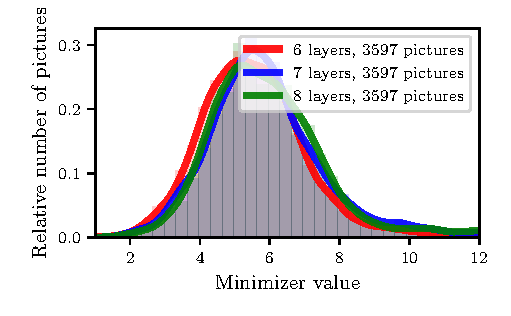
\includegraphics[width = 1\linewidth]{figures/plot_mnist_robustness_minimizer.pdf}
\caption{Comparison of the distribution of the minimized values of different networks for the MNIST dataset.}
\label{fig:comp_min_mnist}
\end{figure}

\begin{figure}
\centering
\showthe\columnwidth
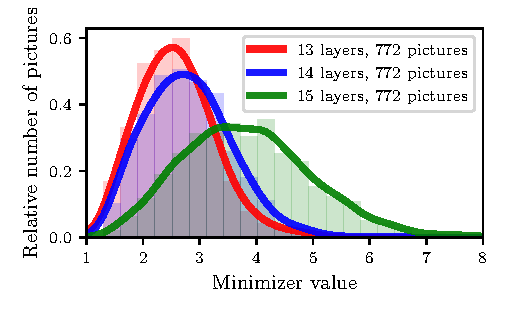
\includegraphics[width = 1\linewidth]{figures/plot_cats_vs_dogs_robustness_minimizer.pdf}
\caption{Comparison of the distribution of the minimized values of different networks for the Cats vs Dogs dataset.}
\label{fig:comp_min_cats_vs_dogs}
\end{figure}

As for the minimize method one cannot compare this rate for a fixed $\epsilon$ as this method does not use such a parameter and does produce the minimal noise for which a misclassification happens. In order to still study this hypothesis, the distribution of the final values of the minimize function \eqref{eq:minimize} were plotted in figure \ref{fig:comp_min_mnist} for the MNIST networks and \ref{fig:comp_min_cats_vs_dogs} for the dogs vs cats networks. Here one yields the same results as with the gradient method. There is no obvious trend for the MNIST networks, however a clear trend for the dogs vs cats networks is noticeable.\\

\section{Conclusion}

As visible in figure \ref{fig:examples} adversarial examples could successfully be created with both presented methods, which are just sightly to not visible at all using the human eye. Overall the minimizer seems to produces better results, as the standard deviation of the noises is in average smaller compared to the onces using the gradient method. This is achieved at the cost of higher computation time. The gradient method produces decent results in short time, while the minimizer produces better results at higher computational cost. \\
The hypothesis of the dependency of the robustness of the networks to the deepness (number of layers) of the networks could not be proven as seen in figure \ref{fig:comp_grad_mnist} \& \ref{fig:comp_min_mnist}. However for the networks trained on the dogs vs cats dataset such a trend was visible (figure \ref{fig:comp_grad_cats_vs_dogs} \& \ref{fig:comp_min_cats_vs_dogs}). In order to actually conclude the truth of this hypothesis, one would need to train a lot more networks with different deepness. As our computational power was limited, this was not possible to us. However we could show that small changes in deepness will not always but can make a change in robustness against adversarial examples.\\
Furthermore, it seems that networks get a lot more vulnerable regarding adversarial examples the large the input dimension is. The dogs vs cats trained networks, which had an input dimension of $(128 \times 128 \times 3)$ produced adversarial examples which were not visible at all, while the MNIST trained networks with an input dimension of $(28 \times 28 \times 1)$ produced noises with which the original shape is still recognizable, however the noise was visible in the adversarial example (figure \ref{fig:examples}).\\


\bibliography{refs}

\section*{Appendix}

\begin{table}
\begin{tabular}{c | c | c}
6 layers & 7 layers & 8 layers  \\ \hline\hline
28x28 CL 32 & 28x28 CL 32 & 28x28 CL 32 \\
28x28 CL 32 & 28x28 CL 32 & 28x28 CL 32 \\
 &   & 28x28 CL 32 \\
2x2 Pool & 2x2 Pool & 2x2 Pool \\
14x14 CL 64 & 14x14 CL 64 & 14x14 CL 64\\
14x14 CL 64 & 14x14 CL 64 & 14x14 CL 64\\
 & 14x14 CL 64 & 14x14 CL 64\\
2x2 Pool & 2x2 Pool  & 2x2 Pool \\
Dropout 0.2 & Dropout 0.2 & Dropout 0.2\\
128 Dense & 128  Dense& 128 Dense\\
10 Output & 10 Output & 10 Output
\end{tabular}
\caption{The design of the different networks for the MNIST dataset. CL means convolutional network followed with the depth (the number of ``maps'') of the layer.  In front of the layer names are written the number of neurons. Pool is a pooling layer, Dense a fully connected, and output the Output layer with a softmax function. The other layers have all rectifier activation functions (ReLu).}
\label{tab:mnist_netw}
\end{table}

\begin{table}
\begin{tabular}{c | c | c}
13 layers & 14 layers & 15 layers  \\ \hline\hline
128x128 CL 32 & 128x128 CL 32 & 128x128 CL 32 \\
128x128 CL 32 & 128x128 CL 32 & 128x128 CL 32 \\
2x2 Pool & 2x2 Pool & 2x2 Pool \\
64x64 CL 64 & 64x64 CL 64 & 64x64 CL 64\\
64x64 CL 64 & 64x64 CL 64 & 64x64 CL 64\\
2x2 Pool & 2x2 Pool  & 2x2 Pool \\
32x32 CL 128 & 32x32 CL 128 & 32x32 CL 128\\
32x32 CL 128 & 32x32 CL 128 & 32x32 CL 128\\
 2x2 Pool & 2x2 Pool  & 2x2 Pool \\
16x16 CL 256 & 16x16 CL 256 & 16x16 CL 256\\
16x16 CL 256 & 16x16 CL 256 & 16x16 CL 256\\
 &  & 16x16 CL 256\\
  2x2 Pool & 2x2 Pool  & 2x2 Pool \\
8x8 CL 256 & 8x8 CL 256 & 8x8 CL 256\\
8x8 CL 256 & 8x8 CL 256 & 8x8 CL 256\\
 & 8x8 CL 256 & 8x8 CL 256\\
 2x2 Pool & 2x2 Pool  & 2x2 Pool \\
256 Dense & 256  Dense& 256 Dense\\
Dropout 0.5 & Dropout 0.5 & Dropout 0.5\\
256 Dense & 256  Dense& 256 Dense\\
Dropout 0.5 & Dropout 0.5 & Dropout 0.5\\
2 Output & 2 Output & 2 Output
\end{tabular}
\caption{The design of the different networks for the Dogs vs Cats data set. The legend is the same as table \ref{tab:mnist_netw}}
\label{tab:dvc_netw}
\end{table}

\end{document}
%
% ****** End of file apssamp.tex ******